% make sure to look for  missing equations in the document
\documentclass[twoside]{article}

\usepackage[math]{kurier}
\usepackage[sc]{mathpazo}
\renewcommand{\sfdefault}{kurier}
\usepackage[boxruled]{algorithm2e}
\usepackage[utf8]{inputenc}
\usepackage[backend=biber]{biblatex}
\usepackage[english]{babel}
\usepackage[english]{babel}
\usepackage[autostyle]{csquotes}
\usepackage{placeins}
\usepackage[a4paper, total={6.5in, 10in}]{geometry}
\usepackage[backend=biber]{biblatex}
\addbibresource{lec_18.bib}

\usepackage{graphics}
\usepackage{graphicx}
\usepackage{subcaption}
\usepackage{amsmath}
\usepackage{float}
\setlength{\oddsidemargin}{0.25 in}
\setlength{\evensidemargin}{-0.25 in}
\setlength{\topmargin}{-0.6 in}
%\setlength{\textwidth}{6.5 in}
%\setlength{\textheight}{8.5 in}
\setlength{\headsep}{0.1 in}
\setlength{\parindent}{0 in}
%\setlength{\cftbeforeequtitleskip}{0pt}
\setlength{\parskip}{1mm plus4mm minus5mm}
%\setlength{\cftafterequtitleskip}{0pt}
\setlength\abovedisplayskip{0mm}


\DeclareMathOperator*{\argmin}{arg\,min}
\DeclareUnicodeCharacter{2212}{-}
\DeclareMathOperator{\EX}{\mathbb{E}}
\newcounter{lecnum}
\renewcommand{\thepage}{\thelecnum-\arabic{page}}
\renewcommand{\thesection}{\thelecnum.\arabic{section}}
\renewcommand{\theequation}{\thelecnum.\arabic{equation}}
\renewcommand{\thefigure}{\thelecnum.\arabic{figure}}
\renewcommand{\thetable}{\thelecnum.\arabic{table}}


\newcommand{\lecture}[3]{
   \pagestyle{myheadings}
   \thispagestyle{plain}
   \newpage
   \setcounter{lecnum}{#1}
   \setcounter{page}{1}
   \noindent
   \begin{center}
   \framebox{
      \vbox{\vspace{2mm}
    \hbox to 6.28in { {\bf \sffamily AA 274: Principles of Robotic Autonomy
                        \hfill Winter 2019} }
       \vspace{4mm}
       \hbox to 6.28in { {\sffamily{\Large \hfill Lecture #1: #2  \hfill}} }
       \vspace{2mm}
       \hbox to 6.28in { {\it Scribes: Adrian Costantino, Behzad Haghgoo, Hubert Lu, Andrew Malty, Peter Schleede, Tane Tatum \hfill} }
      \hbox to 6.28in { {\it Taiming Zhang, and Liuming Zhao \hfill } }
      \vspace{2mm}}
   }
   \end{center}
   \markboth{Lecture #1: #2}{Lecture #1: #2}
   \vspace*{2mm}
}
%%%%%%%%%%%%%%%%%%%%%%%%%%
%document
\begin{document}
\lecture{18}{Decision Making and Dynamic Programming}{}
\vspace{-8mm}
\section{Introduction}
The main objective of this final lecture is to briefly introduce the concept of decision making under uncertainty, which essentially deals with the higher level of the decision making module whereby one is trying to reason about what the other agents in the environment are doing. A useful way of reasoning about the uncertainty of the environment is model the environment as probabilistic problem. This results in the development of control policies that optimize the dynamical system that evolve through time probabilistically.\cite{LEC17}
\section{Basic Decision Making Problem}

\begin{itemize}
    \item We define our \textbf{system} as $$x_{k+1}= f_k(x_k,u_k,w_k), k=0,...,N$$
    Which is very similar to the dynamics studied in the context of filtering in previous sessions.
    \item And we can formalize our \textbf{control constraints} as:
    $$u_k \in U(x_k)$$
    \item And under Markov process assumption, the disturbance the affects the dynamics has a \textbf{probability distribution} that only depends on the current state $x_k$ and current control $u_k$,
    $$P_k(\cdot|x_k,u_k) \ \text{of} \ w_k$$
    \item And are interested in finding a robust closed-loop \textbf{policy} that can be expressed as  $$\pi=\{\mu_0,...,\mu_{N-1}\} \ \text{where} \ u_k=\mu_k(x_k)$$
    which again only depends on the current state.
    \item And we need to have a \textbf{cost} to optimize for. Expected Cost,
    $$J_\pi(x_0)=\EX[g_N(x_N)+\sum_{k=1}^{N-1} g_k(x_k,\mu_k(x_k),w_k)]$$
    Where $g_N$ is the terminal cost and $g_k$ is the stage-wise cost. \\ \\
    Here it is very important to note that we are assuming the cost has an additive structure. This is a plausible assumption and we will that it results in the principle of optimality which will simplify the problem significantly.

    \item And our \textbf{decision making problem} is minimzing this cost and hence can be formulated as
    $$J^\star(x_0)=\min_{\pi} J_\pi(x_0).$$
\end{itemize}
So we can summarize our problem as 
\begin{center}
    \begin{tabular}{|c|c|}
    \hline
        System &  $x_{k+1}= f_k(x_k,u_k,w_k), k=0,...,N$\\
    \hline
        Control Constraints & $u_k \in U(x_k)$ \\
    \hline
        Probability distribution & $P_k(\cdot|x_k,u_k) \ \text{of} \ w_k$ \\
    \hline
        Policy & $\pi=\{\mu_0,...,\mu_{N-1}\} \ \text{where} \ u_k=\mu_k(x_k)$ \\
    \hline
        Expected Cost & $J_\pi(x_0)=\EX[g_N(x_N)+\sum_{k=1}^{N-1} g_k(x_k,\mu_k(x_k),w_k)]$ \\
    \hline
        Decision Making Problem & $J^\star(x_0)=\min_{\pi} J_\pi(x_0)$ \\
    \hline
    \end{tabular}
\end{center}
   
 
\section{Principle of Optimality}
The principle of optimality is a key concept to make stochastic optimal control problem tractable from a computational standpoint. \\
\\
Consider the simplest case (deterministic, i.e. no stochasticity), and suppose the optimal path for a multistage decision-making problem is shown by the figure below
\begin{center}
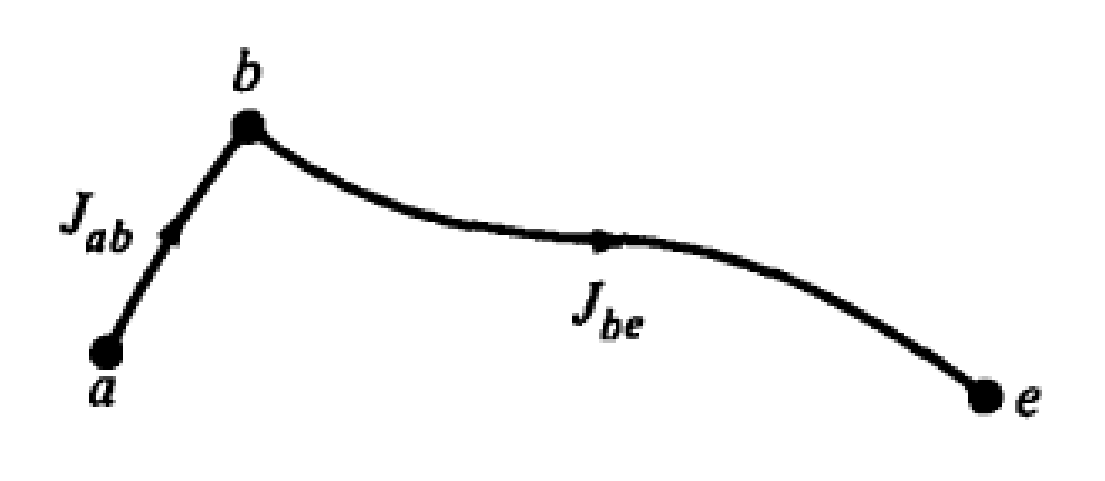
\includegraphics[width=0.5 \textwidth]{image1.png}
\end{center}
where the first decision yields segment $a-b$ with cost $J_{ab}$ , and remaining decisions yield segments $b-e$ with cost $J_{be}$. The total optimal cost is then $J^{\star}_{ae} = J_{ab} + J_{be}$\\
\\
The big claim of the principle of optimality is as follows: if $a-b-e$ is an optimal path from $a$ to $e$, then $b-e$ is an optimal path from $b$ to $e$.
\\
\\
Proof by contradiction: Suppose $b-c-e$ is the optimal path from $b$ to $e$. Then
$$J_{bce} < J_{be}$$
and
$$J_{ab} + J_{bce} < J_{ab} + J_{be}=J^{\star}_{ae}$$
\begin{center}
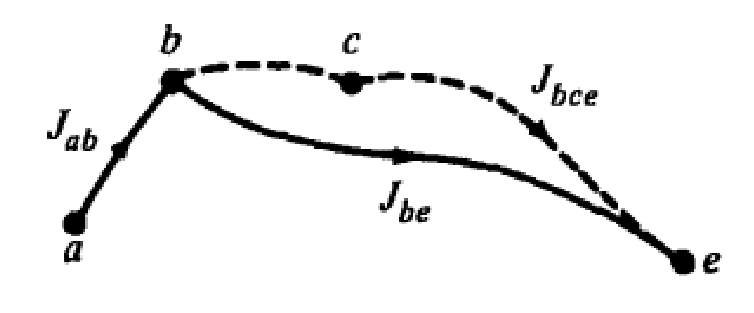
\includegraphics[width=0.5 \textwidth]{image2.png}
\end{center}
This is a contradiction because $J_{be}=J^{\star}_{ae}$ is already defined as the optimal path from $a$ to $e$. If $J_{bce}$ was the optimal path from $b$ to $e$ instead of $J_{be}$, then that would imply that $J^{\star}_{ae}$ is not optimal. Therefore, $J_{be}$ must be the optimal path from $b$ to $e$. \\
\\
\textbf{Remark}: While the principle of optimality holds for tails of optimal policies, the same is not true for heads of optimal policies. Consider the simple game where there are two strategies $\pi_1, \pi_2$. The costs as a function of time for these strategies are
$$r_1(t)=10t $$
$$r_2(t)=e^{0.1t} $$
and the goal of the game is to accumulate as much reward as possible for the duration of the game.
$$\pi^\star_T=\argmin_{i\in\{1,2\}}\sum_{t=1}^{T}$$
It is easy to check that for $T=5$, the optimal policy is $\pi_2$, but if $T=1000$, the optimal policy is $\pi_1$. However, the behavior of $\pi^{\star}_{1000}$ during the first 5 timesteps is not the same as the behavior of $\pi^{\star}_5$.
\\ \subsection{Definition (for discrete-time systems)}
Let $f^\star := \{f_0^\star,f_1^\star, . . . , f_{N−1}^\star \}$ be an optimal policy. Assume state $x_k$ is reachable. Consider the subproblem whereby we are at $x_k$ at time $k$ and we wish to minimize the cost-to-go from time $k$ to time $N$. Then, the truncated policy $\{f_k^\star,f_{k+1}^\star, . . . , f_{N−1}^\star \}$ is optimal for the subproblem.
\\
\\
Considering this definition, tail policies are optimal for tail subproblems. Also, mind that the time-dependence is implicit in the notation: $f_k^\star(x_k)=f^\star(x_k,k)$
\\ \subsection{Applying the principle of optimality}
Consider the problem shown in the figure below.
\begin{center}
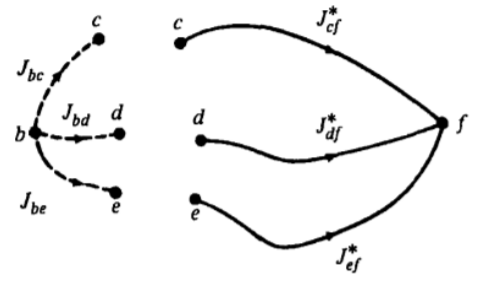
\includegraphics[width=0.5 \textwidth]{image3.png}
\end{center}
According to the principle of optimality, if $b-c$ is the initial segment of the optimal path from $b$ to $f$ , then $c-f$ is the terminal segment of this path. Hence, the optimal trajectory is found by comparing the following:


The comparison of these three trajectories is shown in the figure below.
\begin{center}
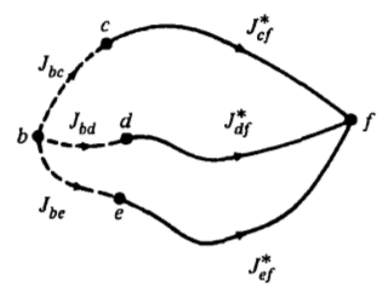
\includegraphics[width=0.5 \textwidth]{image4.png}
\end{center}
When applying the principle of optimality, one only needs to compare the concatenations of immediate decisions and optimal decisions. This provides a significant decrease in the computation required to solve the problem, and also the amount of possible solutions.
\\
\\
In practice, the principle of optimality is applied backward in time. As Soren Kierkegaard said, ``Life can only be understood backwards; but it must be lived forwards."
\\ \subsection{Example problem}
As an example of solving a problem with the principle of optimality, consider the figure below. The goal is to start from node a and end at node h while incurring the minimum cost along the path. Consider the following movement map: [North: UP], [South: DOWN], [East: RIGHT], [West: LEFT].
\\
\begin{center}
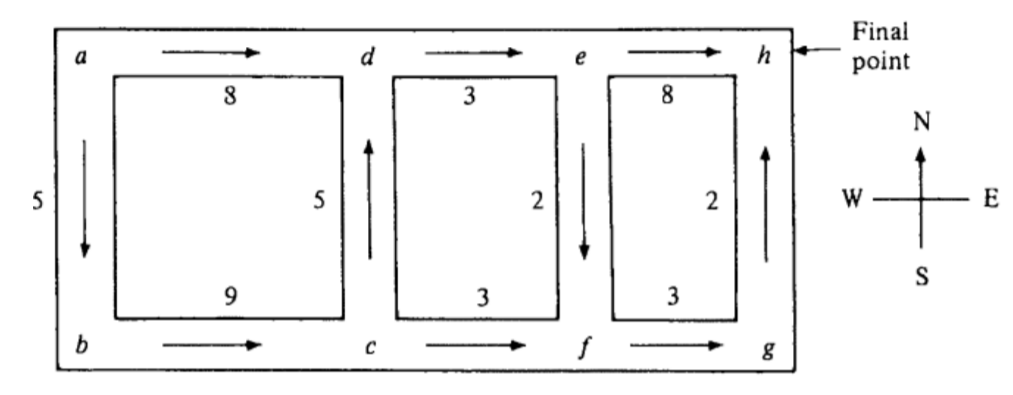
\includegraphics[width= .95 \textwidth]{image5.png}
\end{center}

As mentioned earlier, in practice, the principle of optimality is applied backward in time. First, consider the cost-to-go from starting at node $h:J(h)=0.$ Then, consider the cost-to-go and optimal action for node $ g:J(g)=2+J(h)=2+0=2,u^{\star}(g)=UP$. Continuing for the rest of the problem, we have the following:
\begin{gather*}
J(f)=3+J(g)=3+2=5 \\
u^\star(f) = RIGHT
\end{gather*}
\begin{gather*}
J(e)=\min( 8 + J ( h ) = 8, 2 + J ( f ) = 7 ) = 7 \\
u^\star(e) = DOWN
\end{gather*}
\begin{gather*}
J(d)=3 + J ( e ) = 10 \\
u^\star(d) = RIGHT
\end{gather*}
\begin{gather*}
J(c)=\min( 5 + J ( d ) = 15, 3 + J ( f ) = 8 ) = 8\\
u^\star(c) = RIGHT
\end{gather*}
\begin{gather*}
(b)=9 + J ( c ) = 17 \\
u^\star(b) = RIGHT
\end{gather*}
\begin{gather*}
J(a)=\min ( 5 + J ( b ) = 22, 8 + J ( d ) = 18 ) = 18\\
u^\star(a) = RIGHT
\end{gather*}
Thus, the optimal path for this problem is $a \xrightarrow{} d \xrightarrow{} e \xrightarrow{} f \xrightarrow{} g \xrightarrow{} h.$The optimal cost associated with
this path is $J ( a ) = 18.$

\section{Dynamic Programming (DP) Algorithm}
\\ \subsection{Introduction to DP}
We are given a non linear system with dynamics the following dynamics with additive cost.
\begin{center}
    \[ x_{k+1} = a(x_k, u_k, k) \quad u_k \in U(x_k)   \]
    \[J_f(x_0) = h_N(x_N) + \sum_{k=0}^{N-1} g(x_k, f_k(x_k), k) \]
\end{center}
The dynamic programming algorithm is an algorithm to compute an optimal policy for a dynamic optimization problem that preceeds bacakward in time. We start from the final state
\begin{center}
    \[J_N(x_N) = h_N(x_N)\]
\end{center}
We then move backward and solve the problem of finding the optimal action that trades the immediate cost with the cost to-go, whose cost equation shown below.
\begin{center}
    \[J_k(x_k) = \min_{u_k\in U(x_k)} g_k(x_k, u_k, k) + J_{k+1}(a(x_k, u_k,k)), \quad k = 0,...,N-1  \]
\end{center}
Furthermore, if $u_k^* = f_k^*(x_k)$ minimizes the right hand side of the above equation for each $x_k$ and k, the policy \{$f_0^*, f_1^*,...,f_{N-1}^*$\} is optimal.


For the stochastic case, the situation is very similar except that the cost is the expectation of future stream of random variables. The principle of optimality states that the tail policy is optimal for the tail subproblem where with the tail policy \{$\mu_i^*, ..., \mu_{N-1}^*$\}the tail subproblem is given as
\begin{center}
    \[E\{g_n(x_N) + \sum_{k=i}^{N-1}g_k(x_k,\mu_k(x_k), w_k) \} \]
\end{center}

We fist solve all tail subproblems at the final stage, and at generic step, we solve all tail subproblems of a given time length, using solution of tail subproblems of shorter length. The DP algorithm is similar to what mentioned above. We first start with the final state
\begin{center}
    \[J_N(x_N)=g_N(x_N)\]
\end{center}
and go backwards using
\begin{center}
    \[J_k(x_k)=\min_{u_k\in U_k(x_k)} E_{w_k}\{g_k(x_k, u_k, w_k) + J_{k+1}(f(x_k, u_k, w_k))\}, \quad k = 0, 1, ..., N-1\]
\end{center}
Then $J^*(x_0)=J_0(x_0)$ and optimal policy is constructed by setting $\mu_k^*(x_k)=u_k^*$.

\\ \subsection{Example Problem - Inventory control}
We wish to control the amount of inventory we have across three timesteps $k$. We are given
\begin{align*}
    x_k\in\mathcal{N} &\qquad \text{Stock available at time }k\\
    u_k\in\mathcal{N} &\qquad \text{Inventory purchased at time }k\\
    w_k\in\mathcal{N} &\qquad \text{Demand at time }k.
\end{align*}
The dynamics are simple.
\begin{align*}
    x_{k+1} &= \max(0, x_k+u_k-w_k)
\end{align*}
Put into words, the amount of stock at the next time step is the current stock plus the inventory purchased, minus the demand. However, it can never go below zero. A constraint also keeps the maximum stock plus inventory purchased less than or equal to 2 (which keeps the DP from being too complex).
\begin{align*}
    x_k+u_k\leq 2
\end{align*}
The demand is stochastic, and takes on different values with the probabilities given below.
\begin{align*}
    p(w_k=0)&=0.1\\
    p(w_k=1)&=0.7\\
    p(w_k=2)&=0.2
\end{align*}
	The end cost is 0 for all states and for each timestep $k$, we want to minimize
	\[
	    \mathbf{E}\left\{ u_k+(x_k+u_k-w_k)^2+J_{k+1}(\max(0,x_k+u_k-w_k)) \right\}.
	\]
	This problem clearly has the DP structure, as the cost of a state at a timestep is a function of the cost at the next timestep. As an example, consider the cost of having 0 inventory at $k=2$.
	\begin{align*}
	    J_2(0) &= \underset{u_2=0,1,2}{\text{min}}\mathbf{E}\left\{ u_2+(u_2-w_2)^2 \right\}\\
	    &= \underset{u_2=0,1,2}{\text{min}}\left[ u_2+0.1u_2^2 +0.1(u_2-1)^2 +0.1(u_2-2)^2 \right]\\
	    J_2(0) &= 1.3, \quad \mu_2^*=1
	\end{align*}
When the store owner has no inventory at $k=2$, the best action in this problem is to buy one unit of new inventory. This kind of method can be carried out for all possible states and timesteps. For a small problem like this one, the results can be stored in a lookup table and, based on what happened at each time step, the optimal action can be chosen. This allows the system to respond to stochastic dynamics. However, as will be discussed next, this problem has exponential complexity in terms of number of states $O(n^k)$. As a result, it is often not feasible to compute this exactly. \\

\\ \subsection{Difficulties of DP}
There are essentially three shortcomings associated with Dynamic Programming \\
\begin{enumerate}
    \item \textbf{The Curse of Dimensionality}
    \begin{itemize}
        \item Computational and information storage requirements grow exponentially
        \begin{itemize}
            \item the number of state combinations that must be considered is proportional to the number of possible states raised to the dimension of the problem
        \end{itemize}
        \item In the case of imperfect state information, the problem becomes intractable
        \begin{itemize}
            \item This is often the case for mapping problems, which solves this through the use of partially observable markov decision processes
        \end{itemize}
    \end{itemize}
    \item \textbf{The Curse of Modeling}
    \begin{itemize}
        \item When ”system stochastics” are complex, it is difficult to obtain transition probabilities
    \end{itemize}
    \item \textbf{The Curse of Time}
    \begin{itemize}
        \item Often there is only a short lag time between when enough information is available to compute a solution and when the solution is needed
        \item When the system is subjected to control inputs, state information needed to compute subse- quent solutions may change
        \begin{itemize}
            \item  On-line replanning is required to mitigate this issue
        \end{itemize}
    \end{itemize}
\end{enumerate}
\subsection{Solutions to DP Difficulties: Approximate DP (ADP)}
We can come up with a number of ways to deal with these curses of DP. These methods include
\begin{itemize}
    \item Certainty Equivalent Control 
    \item Cost-to-Go Approximation
    \item Other Approaches (e.g., approximation in policy space)
\end{itemize}
In the following sections we will discuss the first two methods in more detail.
\section{Certainty Equivalent Control (CEC)}\\
	The key concept is to replace a stochastic problem with a deterministic reformulation. Suppose at each time step, k the future uncertain quantities are fixed for some nominal value of those quantities.
	
	We implement the solution on-line in the following way
	
	\begin{itemize}
	    \item for all $i \geq k$, fix $w_i$ at some nominal value $\hat{w}_i$. This leads to a deterministic problem formulation, 
	    \textbf{what is $g_N$ here}
	    \begin{eqnarray*}
	    \min_N g_N(x_N) + \sum_{i = 1}^{N - 1} g_i (x_i, u_i, \hat{w}_i)
	    \end{eqnarray*}
	    where $x_{i + 1} = f_i(x_i, u_i, \hat{w}_i$
	    \item Subsequently, $\mu_k(\hat{x_k})$ is used to control the first element in an optimal control sequence and move to time $k + 1$.
	\end{itemize}


	


{\fontsize{10pt}{12.0pt}\selectfont \textit{where x\textsubscript{i}}\textsubscript{+1} = \textit{f\textsubscript{i}}(\textit{x\textsubscript{i}}, \textit{u\textsubscript{i}}, \textit{w}¯\textit{\textsubscript{i}})}

Subsequently, $ \mu(\bar{x}_k)$ is used to control the first element in an optimal control sequence and move to time k+1.

There are situations were it is, in fact, optimal to replace stochastic quantities with their expected values for the random quantities.\\
For example, if dynamics are linear,noise is guassian, and cost is quadratic is it optimal to replace stochastic quantaties with their expected values.

\section{Cost to Go Approximation (CGA)}
The general idea of cost-to-go approximation is to compute the control input that minimizes the current and expected future cost looking some finite number of time steps ahead. For example, the one step look ahead optimization policy tries to minimize the function:
\begin{align}
    \min_{u_k \in U_k(X_k)}&E(g_k(x_k,u_k,w_k) + \Tilde{J}_{k+1}(f_k(x_k,u_k,w_k))) \\
    \Tilde{J}_N &=g_N \\
    \Tilde{J}_{k+1} &\approx J_{k+1}
\end{align}

$\Tilde{J}_{k+1}$ in the above equation is an approximation of the true cost that is computed in one of several ways discussed below.


\\ \subsection{CGA - Computational Aspects}

Some key points
\begin{itemize}
    \item Assuming $\~J_{k+1}$ is available and minimization isn't difficult, this approach can be implemented on- line, and
    \item Determining an appropriate $\~J_{k+1}$ is highly critical to the output of the approximation
    \begin{itemize}
        \item A simplified surrogate model allows for problem approximation
        \item A parametric formulation computes CGA with a set of tuneable parameters
        \item A rollout approach uses a suboptimal policy to compute $\Tilde{J}_{k+1}$
    \end{itemize}
\end{itemize}
\subsection{Problem Approximation}
Problem approximation allows you to simplify the full system you are trying to solve in order to make an approximate cost simpler to compute. This approach affords us many problem-dependent possibilities. We can,
\begin{itemize}
    \item assume using nominal values in place of uncertainty quantities is sufficiently accurate
    \item create a surrogate model of the problem by ignoring some constraints
    \item assume that subsystem decoupling is non-influential and treat the subsystems independently
    \item use lower resolution solutions of the system by aggregating states together
\end{itemize}

\subsection{Parametric Approximation}
This approach allows for the computation of the CGA based on a parameterization of $\Tilde{J}(x,r)$ where $x$ is the current state and \textit{r }= (\textit{r}\textsubscript{1}, ..., \textit{r\textsubscript{m}}) is a vector of weights that can be tuned \\
\begin{itemize}
    \item it is inherently subjective, because we choose the particular parameterization
    \begin{itemize}
        \item for example: (feature extraction)
        $$\~J_{x,r} = \sum^m_{i=1}r_i y_i(x)$$
        \item Where, $y_i$'s are feature vectors and $\Tilde{J}(x.r)$ is a generic complex function of the state space.
    \end{itemize}
\end{itemize}

\subsection{Rollout}
The cost to go is the optimal cost you would incur if you start at time t+1 at state $x_k +1$ and run an optimal policy from there on.\\
Let's assume you know a policy that isn't optimal, but its decent.  You could approximate the cost by:
\begin{itemize}
    \item start at k+1 
    \item run the policy many times
    \item pin multiple trajectories
    \item average the cost
\end{itemize}
The take away for this approach is the assumption of some heuristic policy referred to as the $"$ base policy$"$.  Implementation of the rollout control approach requires a function definition $ \forall $ \textit{u\textsubscript{k}} $$
\textit{Q\textsubscript{k}}(\textit{x\textsubscript{k}}, \textit{u\textsubscript{k}}) := E  \{  \textit{g\textsubscript{k}}(\textit{x\textsubscript{k}}, \textit{u\textsubscript{k}}, \textit{w\textsubscript{k}}) + \textit{H\textsubscript{k}}\textsubscript{+1}(\textit{x\textsubscript{k}}, \textit{u\textsubscript{k}}, \textit{w\textsubscript{k}}) \}$$ where $H_{k+1}$ is the $"$cost-to-go$"$  value of the base policy and $Q_k$-factors can be:
\begin{itemize}
    \item estimated via Monte Carlo
    \item approximated through a CEC approach
\end{itemize}
Remark: Model Predictive Control (MPC) can be viewed as a special case of a rollout algorithm.



\\ \subsection{Other APD Approaches}
For those that are interested in additional topics to learn about, the following are also useful APD approaches
\begin{itemize}
    \item Minimization of the DP equation error
    \item Direct approximation of the control policies being used
    \item Approximations of the policy space
\end{itemize}

\section{Risk Sensitive Optimization}
As discussed earlier, model uncertainty is an issue when trying to solve for an optimal policy in complex
or probabilistic environments. The goal of this section is to give a brief introduction in how to formulate
cost minimization in a way that is robust to model uncertainty. Recall that we are interested in finding a
policy $\pi^\star$ so that
$$\pi^\star=\argmin_\pi\EX_p[J_\pi(x_0)]$$
where $p$ is a probability distribution that governs the transitions of our system. In many cases, however,
we do not know $p$, so we cannot even evaluate the objective function we wish to minimize. However,
depending on domain knowledge, we may know a set $\Theta$ for which $p\in\Theta$. Here, $\Theta$ is a set of likely
candidates of $p$. Given this knowledge, we can consider the robust formulation

$$\pi^\star=\argmin_\pi\max_{p\in\Theta}\EX_p[J_\pi(x_0)]$$

whereby we aim to minimize our worst case cost over likely transition models in $\Theta$. Note that the risk-neutral situation is a special case of this framework where $\Theta=\{ p \}$.
\\
\\
A few remarks are in order. For general $\Theta$, this problem is intractable. Indeed, if $\Theta$ is discrete lattice of points, then our robust formulation can be casted as an instance of integer programming which is known to be NP hard in the worst case. However, with some regularity conditions on $\Theta$, minimax problems can
be efficiently solved.
\\
\\
\textbf{Definition}: A function $\rho: \mathbb{R}^n \xrightarrow{} \mathbb{R}$ is a \textbf{Coherent Risk measure} if and only if there exists a set $\Theta$ which is a compact, convex subset of all n-dimensional probability vectors such that
$$\rho(v):=\max_{\theta\in\Theta}\theta^Tv$$
While the definition may be abstract, coherent risk measures have several very natural properties. If $\rho: \mathbb{R}^n \xrightarrow{} \mathbb{R}$, then the following hold.
\begin{itemize}
    \item Monotonicity: If $u, v \in \mathbb{R}^n$ are vectors where $u \succeq v$, then $\rho(v) \leq \rho(u)$.
    \item Translation invariance: For $a\in \mathbb{R}, \rho(v+a \textbf{1}=\rho(v)+a$.
    \item Positive homogeneity: If $\lambda > 0 and v \in \mathbb{R}^n$, then $\rho(\lambda v)=\lambda\rho(v)$
    \item Subadditivity: For $u, v \in \mathbb{R}^n$, $rho(u+v) \leq \rho(u) + \rho(v)$
\end{itemize}

The third and fourth properties ensure that $\rho$ is a convex function, meaning that we can minimize coherent risk measures with gradient descent and its variants. If $\Theta$ is a polyhedron, then evaluation of its corresponding coherent risk measure can be done via linear programming.
\\
\\
To wrap things up, we present an example whereby coherent risk measures arise as a natural solution to
an optimization procedure where robustness is desired.
\\
\\
Example: Empirical risk minimization
Consider the standard inference problem whereby $X, Y \sim P$ where $P$ is unknown, and we wish to predict the value of $Y$ given its corresponding value of $X$. For simplicity, let’s say that $X, Y$ are both discrete random variables that can only take on finitely many values $n_x, n_y$ respectively. We are given pairs $\{x_i, y_i\}_{i= 1}^n$ dr
awn i.i.d. from $P$ as training data. One natural thing to try is to pick a loss function $l$, and an estimator $f_\theta$ parameterized by some weights $\theta$, and choose those weights to achieve low loss on the training data. Specifically, we aim to find

\begin{eqnarray*}
    \theta &:=& \arg \min_\theta\sum^n_{i=1}\lamda(\matcal{f}_\theta(\matcal{x}_i),\matcal{y}_i) \\
    &=& \arg \min_\theta \sum_{(x,y)} \hat{P}_n(x,y) \ell (f_\theta(x), y) \\ 
    &=& \arg \min_\theta \mathbb{E}_{\hat{P}_n}[\ell (f_\theta(x), y)]  \\ 
\end{eqnarray*}


Here, $\hat{P}_n$ is the empirical distribution, so that
$$\hat{P}_n(x,y)= \frac{\textrm{The number of times }(x, y) \textrm{ shows up in the training set}}{\textrm{number of training pairs}}$$
However, our true goal is not to do well on the training set, but to be able to generalize on unseen samples coming from $P$. The training set is only useful to us because it gives us some noisy information about thetrue distribution. Thus what we are really interested in is
\begin{eqnarray*}
\theta^* &=& \arg\min_\theta \sum_{(x,y)} P(x,y) \ell(f_\theta (x) , y) \\
&=& \arg\min_\theta \mathbb{E}_p[\ell(f_\theta (X) , Y)]
\end{eqnarray*}
However, this is one particular situation where we do not have knowledge of $P$. We can, however, construct $\Theta$ that will contain $P$ with high probability. If the number of training pairs $n$ is large, we expect that $\hat{P}_n$ will be very similar to $P$. Intuitively, that means if we set $\Theta$ to be the set of probability distributions ``close" to $\hat{P}_n$, then $P$ will be in $\Theta$ with very high probability. By Hoeffding’s Inequality, for any $(x, y)$ we have:
\begin{eqnarray*}
\mathbb{P}\left(|\hat{P}_n(x,y) - P(x,y)| > c\right) \leq \exp\left(-2nc^2\right)
\end{eqnarray*}
Setting $c = \sqrt{\frac{1}{2n}\log(\frac{n_x n_y}{\epsilon})}$ and simplifying the equation, we get
\begin{eqnarray*}
\mathbb{P}\left(|\hat{P}_n(x,y) - P(x,y)| > \sqrt{\frac{1}{2n}\log(\frac{n_x n_y}{\epsilon})}\right) \leq \frac{\epsilon}{n_x n_y}
\end{eqnarray*}

Now union bounding over all $( x, y )$ we get:
\begin{eqnarray*}||\hat{P}_n - P||_\infty \leq \sqrt{\frac{1}{2n} \log \frac{n_x n_y}{\epsilon}}\end{eqnarray*}
with probability at least $1 − \epsilon$. Thus, if we set $\Theta = \{ q \in \Delta^{n_x n_y} : || q − \hat{P}_n|| _{\inf} \leq Cn^{−1/2} \}$ then with high probability, we will have $P \in \Theta$. We can interpret $\Theta$ as a confidence region in the sense that it is extremely unlikely that anything outside of $\Theta$ could have generated our training data, so we do not consider it. Thus if we want to be robust to the fact that our training set is not exactly the same as $P$, we can minimize a coherent risk metric induced by our likely candidates in $\Theta$ as follows:
$$\theta_{CRM}=\arg \min_{\theta}\max_{q\in\theta}\EX[l(f_\theta(X),Y)]$$
\textbf{Remark}: Note that in this example, the set of likely distributions that generated the training data, $ \Theta$, shrinks as the number of training samples $n$ increases. This makes a lot of sense because as you get more data, it is easier to identify the true distribution, thus the need to be robust is lessened. A similar phenomenon can be observed between frequentist and Bayesian estimators. When the number of samples is small, the Bayesian prior has a significant effect on the estimation, but as the number of samples grows, the frequentist and Bayesian estimators converge to one another.

\printbibliography

\subsubsection*{Contributors}
Winter 2019: Adrian Costantino, Behzad Haghgoo, Hubert Lu, Andrew Malty, Peter Schleede, Tane Tatum, Taiming Zhang, and Liuming Zhao   \\
Winter 2018: Michal Adamkiewicz, Scott Park, Adrian Piedra, Garrett Taylor,and Matthew Wu Tsao  

\end{document}